\documentclass[12pt]{Report}

\usepackage{graphicx}

%opening
\title{The Best Option for Writing TDDs at FINCAD}
\author{Bruce Krayenhoff}

\begin{document}

\maketitle

\begin{abstract}
At FINCAD we write TDDs (Technical Design Documents) before implementing any project or production-quality code.  
The language or tool used to write these TDDs is not specified, however it must be saved as plain text so that it is 
compatible with version control and code-review systems.

In addition to these requirements, it is desirable to use a tool that is familiar to FINCADIANs, and allows us to easily express and tweak our ideas.

So far the language most commonly used for TDDs is HTML, with some quants and financial engineers using IPython Notebook.

In this report we consider HTML, Markdown, Python, Latex, and IPython Notebook as options for writing TDDs.  
I shall argue that IPython Notebook and possibly Markdown have many advantages and merit experimentation for use in TDDs and elsewhere.
\end{abstract}

\section{Introduction}
Previously a programmer would just go at a project themselves, then incorporate the feedback of others at code-review stage.  
This would result in much wasted time as programmers refactored to incorporate this feedback. 
In recent years, FINCAD has moved toward extensively documenting planned projects in TDDs (Technical Design Documents), 
which are review and signed-off on before the programmer commences production quality code.  
As a result, less time is spent coding and refactoring, while a substantial amount of time is spent in design, including drafting and modifying a TDD.

When I first commenced writing a TDD I learned some HTML and programmed in HTML directly. 
This was painstakingly time-consuming, hence I looked at several alternatives, which are the subject of this report.  
The alternatives considered are:

\begin{enumerate}
	\item HTML, CSS, and Javascript
	\item Markdown, augmented by HTML and CSS
	\item Python
	\item Latex
	\item IPython Notebook
\end{enumerate}

We will narrow down the options to HTML, Markdown, and IPython Notebook then compare them using several desiderata.


\section{The Options}

\subsection{HTML, CSS, and Javascript - Qualifies}
	\paragraph{Advantages}
	%subsubsection{Advantages}
		HTML documents have the advantage that anyone can easily view them, since everyone has a Browser.  
		Also, most programmers have some familiarity with HTML, and many text editors and IDEs have excellent support for HTML.  
		Also, KompoZer has an excellent WYSIWYG interface to HTML that produces very read-able HTML code.  
		HTML, CSS, and Javascript are what we make webpages out of, so they provide great flexibility!
	\paragraph{Disadvantages}
	%\subsubsection{Disadvantages}
		With all its tags, HTML code is harder to read and edit than Markdown (See Fig. \ref{HTML code}).  
		Aided by Javascript, it can syntax highlight code when rendered, but not during editing.  
		The main disadvantage of HTML, therefore, is that it isn't as easy to edit as other formats, particularly when editing the code directly.
		\begin{figure}[h]
			\centering
			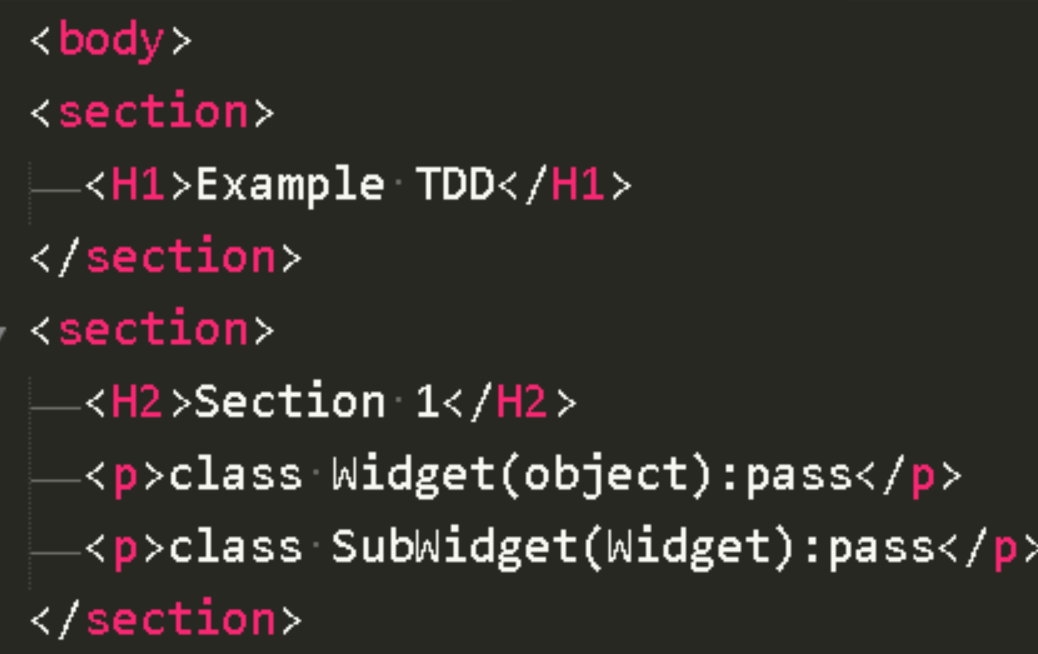
\includegraphics[scale=.25]{HTML_code.PNG}
			\caption{Some HTML code}
			\label{HTML code}
		\end{figure}
		

\subsection{Markdown - Qualifies}
	%\subsubsection{Advantages}
	\paragraph{Advantages}
	Markdown has one aspect in which it really shines: The read-ability of its code.  
	This would make working directly with the code, code reviews, and diffs in version control systems easier.  
	Also, when the syntax of markdown is insufficient, one can augment it with HTML, CSS, etc.  
	Github flavored markdown can also easily do syntax highlighting of code.  
	Finally, Stackedit and MarkdownPad are both excellent mardown editors that support Github flavored markdown, 
	show instant previews, and allow you to work offline (See Fig. \ref{StackEdit}).
	
	\begin{figure}[h]
		\centering
		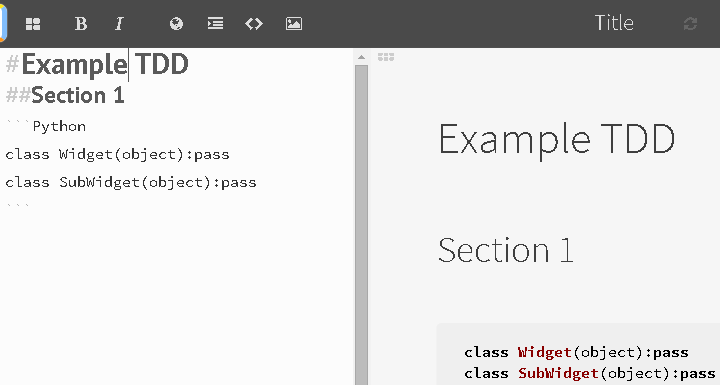
\includegraphics[scale=.5]{StackEdit.png}
		\caption{Editing Markdown Using StackEdit}
		\label{StackEdit}
	\end{figure}
	
	%\subsubsection{Disadvantages}
	\paragraph{Disadvantages}	
	Markdown has drawbacks. It would need to be converted to HTML or a special program is needed for viewing nicely rendered documents.  
	There isn't the same support for markdown in text editors and IDEs as is available for HTML/CSS alone.  
	Also, there are multiple flavours of markdown, which could lead to compatibility problems unless a flavour, 
	such as Github flavored markdown, were chosen as the standard within FINCAD.


\subsection{Python - Eliminated}
	Python is already used as a complement to TDDs, though not as a TDD itself.
	%\subsubsecction{Advantages}
	\paragraph{Advantages}
		The biggest advantage of using a Python file for at least part of a TDD 
	is that editors/IDEs can provide syntax highlighting and autocompletion of the Python code.
	
	%\subsubsection{Disadvantages}
	\paragraph{Disadvantages}	
	The major dis-advantage is the lack of flexibility.  Creating titles in a larger fonts and tables appears to be impossible.  
	Python code is a useful complement or include for a TDD, but does not provide sufficient flexibility to be used alone.  
	Hence, \emph{I exclude Python from consideration in the remainder of this document}.


\subsection{Latex - Eliminated}
	%\subsubsection{Advantages}
	\paragraph{Advantages}
	
	Many Quants are familiar with Latex to format documents, and in particular mathematical equations.
	
	Latex's strength is in formatting mathematical equations and publishable documents.  
	However HTML and IPython can also format mathematical equations, and TDDs need only be easy to understand, not formatted to publish.
	
	%\subsubsection{Disadvantages}
	\paragraph{Disadvantages}	
	A major disadvantage of Latex is that it would be totally unfamiliar to many programmers at FINCAD, 
	and I expect they would be unwilling to use Latex when HTML is familiar and likely to be much more useful in their future careers.
	
	For this reason, because I have not heard of TDDs ever being written using Latex, and because I am not that familiar with Latex myself, 
	\emph{I exclude Latex from consideration in the remainder of this document}.


\subsection{IPython Notebook - Qualifies}
	%\subsubsection{Advantages}
	\paragraph{Advantages}
		IPython Notebook is an incredibly flexible jack-of-all-trades.  
		You can type Python code with syntax highlighting and autocomplete support. 
		You can then run the code, including the outputted text or graphs in your TDD.  
		Your IPython notebook can include and render Markdown, HTML/CSS, and Latex code (See Fig. \ref{IPython}).  
		You can export to HTML, Latex, and other formats.  
		You can even, with a simple command, copy Python, Markdown, Latex, or HTML code from a file into IPython Notebook.
		
		IPython Notebook is commonly edited through a browser-based client as depicted in figure \ref{IPython}.  However, clients exist for editing IPython Notebooks inside editors such as Sublime Text, Pycharm, and Emacs, so you can continue to use your favorite programming environment!
		
		\begin{figure}[h]
			\centering
			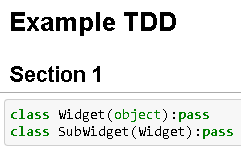
\includegraphics[scale=.75]{IPython_Notebook.PNG}
			\caption{Editing an IPython Notebook}
			\label{IPython}
		\end{figure}
		
		Finally, IPython may be useful more generally and therefore worth learning.  
		For instance, IPython Notebook's interactive computing abilities could be used for building Excel workbooks 
			using the Workbook Description Language I am designing.
		Also, IPython serves as an excellent terminal and shell scripting language, allowing you to almost seamlessly mix Python and Shell commands.
		
	%\subsubsection{Disadvantages}
	\paragraph{Disadvantages}	
		While IPython Notebook is a jack-of-all-trades, it is a master of none.  
		I would definitely prefer to edit HTML in KompoZer, Markdown in StackEdit, Latex in TeXstudio, and Python in PyCharm.  
		And while IPython allows you to easily copy files edited in these other programs into you IPython Notebook, I don't know how to completely automate this.
		
		Furthermore, while IPython Notebook is stored as a JSON text file and can thus be diffed and code-reviewed, 
		this JSON file has lots of boiler-plate text that makes it difficult to read (See Fig. \ref{IPython_JSON}).
		
		\begin{figure}[h]
			\centering
			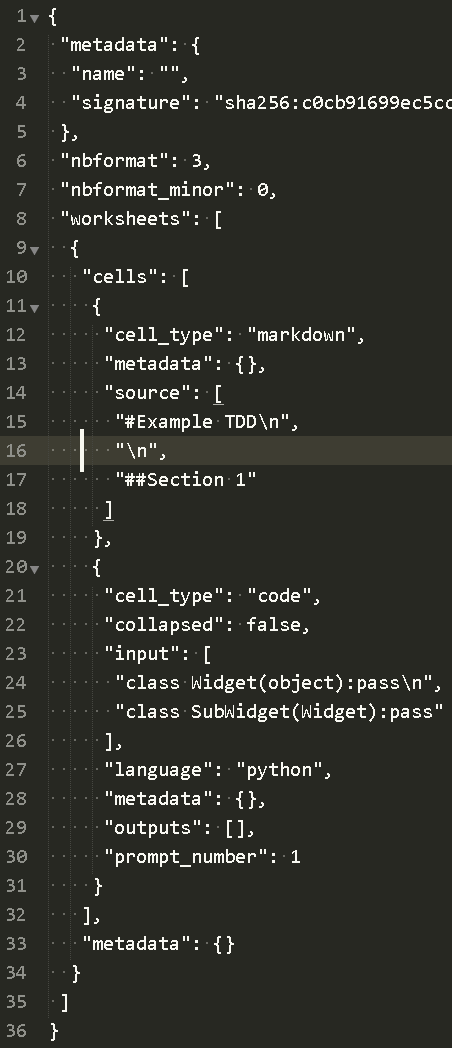
\includegraphics[scale=.45]{IPython_Notebook_code.PNG}
			\caption{The JSON file underlying the IPython Notebook of Figure \ref{IPython}}
			\label{IPython_JSON}
		\end{figure}
		
		


\section{Comparison and Discussion}
We have 3 remaining options that qualify so far: HTML, Markdown, and IPython Notebook.

We have the following requirements and desiderata for creating TDDs:

\begin{enumerate}
	\item Requirements:
		\begin{enumerate}
			\item Amenable to code review
			\item Amenable to version control
		\end{enumerate}
	\item Desiderata:
		\begin{enumerate}
			\item Familiar
			\item Easy to use
			\item Easy to view
			\item Capable of expressing the ideas that we wish to convey			
		\end{enumerate}
\end{enumerate}

Out of the remaining options, all of them are amenable to code review and version control because they are stored in plain text.  
Markdown is the easiest to do diffs and code review because it is easiest to work with as plain text.  
IPython Notebook is the hardest.  However, code reviews are usually only comprise a small part near the end of the design process, 
in which the design is officially signed off on.  Working with diffs probably comprise only a small fraction of the time spent working on a TDD.  
Hence ease is of secondary importance for diffs and version control.

As a software engineering firm, I'm sure we will be able to easily surmount any difficulties with viewing whatever options we choose.  
Since they can all render HTML/CSS code, I'm sure that the remaining options all have sufficient expressive power.

This leaves us with 2 dimensions along which to differentiate the options: Familiarity and ease of use.


\subsection{Familiarity}
HTML is probably the most familiar option, although many programmers are familiar with markdown 
(A flavour is used for the FINCAD wiki!).  IPython would involve a learning curve for most.  In fact, I discussed 
IPython Notebook with one of the quants that is using it, and he was not familiar some functionality that 
would have been very useful for him!

\subsection{Ease of Use}
The ease of use depends on the task you want to accomplish:
\begin{description}
	\item[Python] 
		If you want syntax highlighted Python code, IPython is easiest because it provides autocomplete and syntax highlighting while 
		you edit, rather than applied later.  Alternatively, IPython Notebook can easily import from a file created in your favorite Python editor.  Also, IPython notebook can automatically include graphs from MatPlotLib Python code (Which is valuable for quants).
	\item[Rich Text] 
		If you want to create bold and italisized text with different font sizes through a WYSIWYG interface, HTML or Markdown is best.
	\item[Colors and Highlighting] 
		If you want to view font colors and highlighting as you edit, a good WYSIWYG HTML editor like KompoZer is your best bet.
	\item[Emacs]
		If you want to stick with you favorite text editor such as Emacs, Markdown's easy-to-read syntax may be your best choice, or you can try the IPython Notebook client for you text editor.
\end{description}
	




\section{Recommendations}
	IPython and possibly Markdown have significant advantages over HTML, and also some drawbacks, some of which may not be clear at this point.  
	IPython also requires a moderate time investment to learn.  Give this cost and the uncertainty of the benefits, it is premature to encourage 
	everyone to start using an option other than HTML.  However given the amount of time that is spent in design and the possibly significant 
	advantages of IPython, experimentation by early adopters should be encouraged by raising awareness of these options.
	
	By experimenting with and finding the best tools for the job, 
	we can save developers time during the design phase and accelerate software development at FINCAD!
	
\end{document}

















